% Technical project report - Mini Automotive ECU Network with UDS Diagnostics
% Build: latexmk -xelatex main.tex   (XeLaTeX + biber)
\documentclass[a4paper,12pt]{report}
\setcounter{tocdepth}{2}
\PassOptionsToPackage{colorlinks=true,linkcolor=black,citecolor=black,urlcolor=blue,unicode}{hyperref}
\usepackage{geometry}
\geometry{a4paper, left=30mm, top=25mm, bottom=20mm, right=20mm}
\usepackage{amsfonts}
\usepackage{amsmath}
\usepackage{enumitem}
\usepackage{xcolor}
\usepackage[toc]{appendix}
\usepackage{graphicx}
\usepackage{mathtools}
\usepackage[labelfont=bf]{caption}
% ── Unicode font setup (XeLaTeX) ──────────────────────────────
\usepackage{fontspec}
\setmainfont{Latin Modern Roman}
\setsansfont{Latin Modern Sans}
\setmonofont{lmmono10-regular.otf}[
  Scale=MatchLowercase,
  ItalicFont=lmmono10-italic.otf,
  BoldFont=lmmonolt10-bold.otf,
  BoldItalicFont=lmmonolt10-boldoblique.otf
]
\usepackage[english]{babel}
\usepackage{csquotes}
\usepackage{float}
\usepackage{makecell}
\usepackage{ragged2e}
\usepackage{longtable}
\usepackage{booktabs}
\usepackage{subcaption}
\usepackage{placeins}
\usepackage{tocloft}
\makeatletter
\renewcommand{\@makeschapterhead}[1]{%
  \vspace*{10\p@}%
  {\parindent \z@ \raggedright \normalfont
   \interlinepenalty\@M
   \Huge \bfseries #1\par\nobreak
   \vskip 18\p@}}
\makeatother
\renewcommand{\cftfigfont}{\small}
\renewcommand{\cftfigpagefont}{\small}
\renewcommand{\cfttabfont}{\small}
\renewcommand{\cfttabpagefont}{\small}
\setlength{\cftbeforefigskip}{0pt}
\setlength{\cftbeforetabskip}{0pt}
\usepackage{tikz}
\usetikzlibrary{shapes.geometric, arrows.meta, positioning, fit, backgrounds, calc, decorations.pathreplacing}
\usepackage{listings}
\usepackage{microtype}
\usepackage{array}
\usepackage{multirow}
\usepackage{tabularx}
\usepackage{pifont}
\usepackage[style=ieee,backend=biber,sorting=none,doi=true,url=true,isbn=false]{biblatex}
\AtEndPreamble{%
  \ifundef{\abx@macro@volume+number}%
    {\newbibmacro*{volume+number}{}}%
    {}%
}
\addbibresource{reference.bib}
\usepackage{xurl}
\usepackage{hyphenat}
\usepackage{hyperref}
\newcommand{\cmark}{\ding{51}}
\newcommand{\xmark}{\ding{55}}
\newlist{tblitem}{itemize}{1}
\setlist[tblitem]{label=\textbullet, nosep, leftmargin=1.1em, itemsep=0pt, topsep=0pt, partopsep=0pt, parsep=0pt}
\newcommand{\reportimage}[4]{%
  \begin{figure}[H]
    \centering
    \includegraphics[width=#2\textwidth]{images/#1}
    \caption{#3}
    \label{#4}
  \end{figure}
}
\usepackage{etoolbox}
\AtBeginEnvironment{figure}{\captionsetup{font=small}}
% ── Code listing style ────────────────────────────────────────
\definecolor{codebg}{RGB}{245,245,245}
\definecolor{codegreen}{RGB}{0,128,0}
\definecolor{codegray}{RGB}{128,128,128}
\definecolor{codeblue}{RGB}{0,0,200}
\lstdefinestyle{mystyle}{
  backgroundcolor=\color{codebg},
  commentstyle=\color{codegreen},
  keywordstyle=\color{codeblue}\bfseries,
  numberstyle=\tiny\color{codegray},
  stringstyle=\color{orange},
  basicstyle=\ttfamily\footnotesize,
  breakatwhitespace=false,
  breaklines=true,
  captionpos=b,
  keepspaces=true,
  numbers=left,
  numbersep=5pt,
  showspaces=false,
  showstringspaces=false,
  showtabs=false,
  tabsize=2,
  frame=single,
  rulecolor=\color{gray!40},
  language=C
}
\lstset{style=mystyle}
\microtypesetup{protrusion=true,expansion=false}
\setcounter{secnumdepth}{2}
\AtBeginDocument{%
  \renewcommand{\contentsname}{TABLE OF CONTENTS}%
  \renewcommand{\listfigurename}{LIST OF FIGURES}%
  \renewcommand{\listtablename}{LIST OF TABLES}%
}
\setlength{\emergencystretch}{6em}
\pretolerance=1000
\tolerance=2000
\Urlmuskip=0mu plus 1mu\relax
\raggedbottom
% ── TikZ styles shared by the diagrams ────────────────────────
\tikzset{
  box/.style={draw, rounded corners=3pt, align=center, font=\small, inner sep=5pt},
  node/.style={box, fill=blue!6, minimum width=3.6cm, minimum height=1.4cm},
  layer/.style={box, minimum width=9.5cm, minimum height=0.9cm},
  arr/.style={-{Stealth[length=2.2mm]}, thick},
}
\begin{document}
\begin{titlepage}
    \begin{center}
        \vspace*{2.5cm}

        \Large
        PERSONAL PROJECT REPORT

        \vspace{2.0cm}

        \Huge
        \textbf{Mini Automotive ECU Network with UDS Diagnostics}\\[0.8cm]
        \Large
        CAN communication, end-to-end protection and ISO-TP on an\\
        STM32G4 Sensor ECU and an STM32MP157 Control ECU

        \vspace{2.4cm}

        \Large
        By\\
        \textbf{Tu Dinh Huy}

        \vspace{1.2cm}

        \large
        Interim report -- milestones M1 to M5\\[0.3cm]
        Source code: \url{https://github.com/huydinhischanging/mini-automotive-ecu-uds}\\[0.1cm]
        Demo video: \url{https://www.youtube.com/watch?v=Ocq1K0BO8kM}

        \vfill
        Ho Chi Minh City, Vietnam\\
        September 2026

    \end{center}
\end{titlepage}

\clearpage
\tableofcontents{}
\clearpage
{\renewcommand{\addvspace}[1]{\vspace{2pt}}\listoffigures}
\addcontentsline{toc}{chapter}{LIST OF FIGURES}
\clearpage
{\renewcommand{\addvspace}[1]{\vspace{2pt}}\listoftables}
\addcontentsline{toc}{chapter}{LIST OF TABLES}
\clearpage
\chapter*{LIST OF ABBREVIATIONS}
\addcontentsline{toc}{chapter}{LIST OF ABBREVIATIONS}

{\small
\renewcommand{\arraystretch}{0.9}
\begin{longtable}{@{}p{3.2cm} p{11cm}@{}}
\textbf{ACK}      & Acknowledge (CAN bit acknowledging a correctly received frame) \\
\textbf{ADC}      & Analog-to-Digital Converter \\
\textbf{AUTOSAR}  & AUTomotive Open System ARchitecture \\
\textbf{BS}       & Block Size (ISO-TP flow-control parameter) \\
\textbf{CAN}      & Controller Area Network \\
\textbf{CCU}      & Clock Calibration Unit (of FDCAN1 on the STM32MP1) \\
\textbf{CF}       & Consecutive Frame (ISO-TP) \\
\textbf{CRC}      & Cyclic Redundancy Check \\
\textbf{DLC}      & Data Length Code \\
\textbf{DTC}      & Diagnostic Trouble Code \\
\textbf{E2E}      & End-to-End (communication protection) \\
\textbf{ECU}      & Electronic Control Unit \\
\textbf{FC}       & Flow Control frame (ISO-TP) \\
\textbf{FDCAN}    & Flexible Data-rate CAN controller (ST implementation of Bosch M\_CAN) \\
\textbf{FF}       & First Frame (ISO-TP) \\
\textbf{HAL}      & Hardware Abstraction Layer (STM32Cube) \\
\textbf{HSE}      & High-Speed External oscillator \\
\textbf{HSI}      & High-Speed Internal RC oscillator \\
\textbf{ISO-TP}   & ISO 15765-2 transport protocol \\
\textbf{ISR}      & Interrupt Service Routine \\
\textbf{LSB}      & Least Significant Bit \\
\textbf{MCAL}     & Microcontroller Abstraction Layer (AUTOSAR) \\
\textbf{MCU}      & Microcontroller Unit \\
\textbf{MPU}      & Microprocessor Unit \\
\textbf{NBT}      & Nominal Bit Time, in time quanta \\
\textbf{NRC}      & Negative Response Code (UDS) \\
\textbf{PLL}      & Phase-Locked Loop \\
\textbf{PWM}      & Pulse-Width Modulation \\
\textbf{RTOS}     & Real-Time Operating System \\
\textbf{SF}       & Single Frame (ISO-TP) \\
\textbf{SJW}      & Synchronisation Jump Width \\
\textbf{SP}       & Sample Point \\
\textbf{STmin}    & Minimum Separation Time between consecutive frames (ISO-TP) \\
\textbf{tq}       & Time quantum \\
\textbf{UART}     & Universal Asynchronous Receiver-Transmitter \\
\textbf{UDS}      & Unified Diagnostic Services (ISO 14229) \\
\end{longtable}
}
\pagebreak

\clearpage
\chapter*{ABSTRACT}
\addcontentsline{toc}{chapter}{ABSTRACT}

This report describes the design and the first two milestones of a scaled-down in-vehicle network built from low-cost development boards. A \textit{Sensor ECU} on an STM32G431 (NUCLEO-G431RB) samples a potentiometer that emulates vehicle speed and publishes it on a 500\,kbit/s classic CAN bus every 10\,ms. A \textit{Control ECU} runs FreeRTOS on the Cortex-M4 core of an STM32MP157D (STM32MP157D-DK1), next to Linux on the Cortex-A7 cores, and consumes the signal, monitors it for faults and drives a PWM output. A diagnostic tester using UDS (ISO~14229) over ISO-TP (ISO~15765-2) completes the target architecture.

The software follows an AUTOSAR-inspired layering in which only the MCAL layer touches the vendor HAL. Protocol modules (ISO-TP, end-to-end protection with an alive counter and CRC-8 SAE-J1850) are written in portable C and are tested on a PC with a small fault-injection-capable test harness: 34 unit tests with 173 checks pass, including a 4095-byte ISO-TP transfer between two protocol instances.

Both ECUs were verified on hardware in FDCAN internal loopback. The Sensor ECU sent more than 59\,000 frames at the designed 110\,frames/s with no dropped frame and no bus-off; the ADC reading was stable to $\pm$1--2\,LSB. The Control ECU processed 30\,900 frames with zero CRC, sequence or queue-overflow errors while its output tracked the received speed. Bringing up the Control ECU uncovered two platform issues that were diagnosed by reading M4 memory and peripheral registers from Linux, without a hardware debugger: a SysTick handler missing from STM32CubeMX-generated code, and an FDCAN kernel clock stuck in a glitch-free multiplexer whose previous input had been disabled by Linux.

The remaining milestones are the physical two-node bus, the UDS server with DTC management, and a Python tester on Linux.

\bigskip
\noindent\textbf{Keywords:} Controller Area Network, ISO-TP, UDS, AUTOSAR E2E, STM32MP157, FreeRTOS, embedded C, unit testing.
\newpage

\clearpage
\chapter{INTRODUCTION}
\label{ch:intro}

\section{Background}

A modern vehicle contains dozens of electronic control units (ECUs) that exchange data over in-vehicle networks, most commonly the Controller Area Network (CAN)~\cite{ISO11898-1}. Each ECU samples sensors, runs control software and, just as importantly, supervises itself: it detects missing or implausible signals, stores diagnostic trouble codes (DTCs) and answers a workshop tester through a standardised diagnostic protocol, Unified Diagnostic Services (UDS)~\cite{ISO14229-1}. Because a CAN frame carries at most eight data bytes, diagnostic messages travel over the ISO-TP transport layer, which segments and reassembles longer messages~\cite{ISO15765-2}.

These building blocks, deterministic communication, end-to-end protection of safety-relevant signals, fault management and diagnostics, are the daily material of automotive embedded software. They are rarely visible in hobby projects, which usually stop at reading a sensor and blinking a LED.

\section{Problem Statement and Motivation}

Professional automotive tool chains (AUTOSAR stacks, commercial CAN analysers, production ECUs) are expensive and hide most of the mechanisms behind configuration tools. A learner therefore has few opportunities to implement and debug the protocols end to end on real hardware. The goal of this project is to build a miniature but technically faithful ECU network from affordable development boards, implementing the protocols from the standards rather than from vendor black boxes, and to document the engineering decisions in a way that can be reviewed.

\section{Objectives}

\begin{enumerate}[label=\textbf{O\arabic*.}]
  \item Build a two-ECU classic CAN network at 500\,kbit/s with a correct, justified bit-timing configuration on two different STM32 families.
  \item Protect the cyclic sensor signal end to end (alive counter and CRC) and detect timeout, out-of-range and corrupted data at the receiver, with a defined safe state.
  \item Implement ISO-TP and a UDS server (sessions, tester present, read data by identifier, read and clear DTCs, ECU reset, negative responses) on the Control ECU.
  \item Structure the firmware in AUTOSAR-like layers so that protocol code is hardware independent and unit tested on a PC.
  \item Run the Control ECU on the Cortex-M4 of a heterogeneous STM32MP157, alongside Linux, as in modern domain controllers.
\end{enumerate}

\section{Scope of this Report}

This is an interim report. Table~\ref{tab:status} summarises what is complete and verified at the time of writing. All results in Chapter~\ref{ch:results} refer to the completed items only; the remaining items are described as design and future work.

\begin{table}[H]
\centering
\small
\caption{Project status at the time of writing}
\label{tab:status}
\begin{tabularx}{\textwidth}{@{}p{7.2cm}Xc@{}}
\toprule
\textbf{Work item} & \textbf{Evidence} & \textbf{Status} \\
\midrule
Sensor ECU firmware (ADC, cyclic CAN, E2E, fault injection) & M1 hardware test & \cmark \\
ISO-TP transport layer & 26 unit tests & \cmark \\
E2E protection library (shared by both ECUs) & 8 unit tests & \cmark \\
Control ECU firmware on the Cortex-M4 (FreeRTOS, E2E check, fault monitor, safe-state output) & M2 hardware test & \cmark \\
Two-node physical CAN bus with transceivers & -- & planned (M3) \\
UDS server and DTC manager & -- & planned \\
Python tester on Linux (SocketCAN) & -- & planned \\
Static analysis (cppcheck/MISRA) and demo video & -- & planned \\
\bottomrule
\end{tabularx}
\end{table}

\section{Report Structure}

Chapter~\ref{ch:background} reviews the relevant protocols and the STM32MP1 heterogeneous architecture. Chapter~\ref{ch:design} presents the hardware, the CAN configuration and the software design of both ECUs. Chapter~\ref{ch:results} reports the implementation, the unit tests and the two hardware milestones, including the diagnosis of two bring-up issues. Chapter~\ref{ch:discussion} evaluates the results against the objectives and discusses limitations, and Chapter~\ref{ch:conclusion} concludes with the remaining work. The appendices contain the frame layouts and the build and diagnosis procedures.

\chapter{TECHNICAL BACKGROUND}
\label{ch:background}

This chapter summarises the standards and platform features that the design relies on. It is not a complete tutorial; the cited specifications are normative.

\section{Controller Area Network}

CAN is a multi-master serial bus with non-destructive bitwise arbitration: when several nodes start transmitting, the frame with the lowest identifier wins and the others retry automatically~\cite{BoschCAN20,ISO11898-1}. Every receiver acknowledges a correct frame in the ACK slot, so a transmitter that is alone on the bus sees an acknowledgement error and keeps retrying. Each node maintains transmit and receive error counters; above 255 transmit errors it enters the \textit{bus-off} state and stops participating until it has observed 128 occurrences of 11 recessive bits.

\subsection{Bit timing}

A bit is divided into time quanta (tq) of length $t_q = \text{prescaler} / f_\text{kernel}$. The nominal bit time is
\begin{equation}
  \text{NBT} = 1 + \text{Seg1} + \text{Seg2} \quad [\text{tq}], \qquad
  \text{bitrate} = \frac{f_\text{kernel}}{\text{prescaler}\cdot\text{NBT}},
\end{equation}
where the leading quantum is the synchronisation segment, Seg1 combines propagation and phase segment 1, and Seg2 is phase segment 2. The bus is sampled at the sample point
\begin{equation}
  \text{SP} = \frac{1 + \text{Seg1}}{\text{NBT}},
\end{equation}
for which automotive networks typically use about 87.5\,\%. The synchronisation jump width (SJW) limits how far a node may re-align its bit phase on each recessive-to-dominant edge. Because every node samples with its own oscillator, the tolerated clock deviation is bounded by~\cite{ISO11898-1}
\begin{equation}
  \Delta f \le \min\left( \frac{\text{SJW}}{20\,\text{NBT}},\;
  \frac{\min(\text{Seg1},\text{Seg2})}{2\,(13\,\text{NBT} - \text{Seg2})} \right).
  \label{eq:tolerance}
\end{equation}
For the configurations in this project the bound is below 0.5\,\%, which rules out on-chip RC oscillators (typically $\pm$1\,\%) and motivates crystal clocks on both ECUs.

\section{ISO-TP (ISO 15765-2)}

ISO-TP transports messages of up to 4095 bytes over classic CAN frames~\cite{ISO15765-2}. The first byte (protocol control information) identifies four frame types:
\begin{itemize}[nosep]
  \item \textbf{Single Frame (SF)} \texttt{0L}: up to 7 data bytes.
  \item \textbf{First Frame (FF)} \texttt{1L LL}: 12-bit total length and 6 data bytes.
  \item \textbf{Consecutive Frame (CF)} \texttt{2N}: 7 data bytes with a 4-bit sequence number that wraps from 15 to 0.
  \item \textbf{Flow Control (FC)} \texttt{3S BS STmin}: sent by the receiver with a flow status (continue, wait, overflow), a block size BS (number of CFs before the next FC, 0 = unlimited) and the minimum separation time STmin between CFs.
\end{itemize}
Timers supervise the exchange: the sender waits at most N\_Bs for a flow control, the receiver at most N\_Cr for the next consecutive frame. Figure~\ref{fig:isotp_seq} shows a segmented transfer.

\begin{figure}[H]
\centering
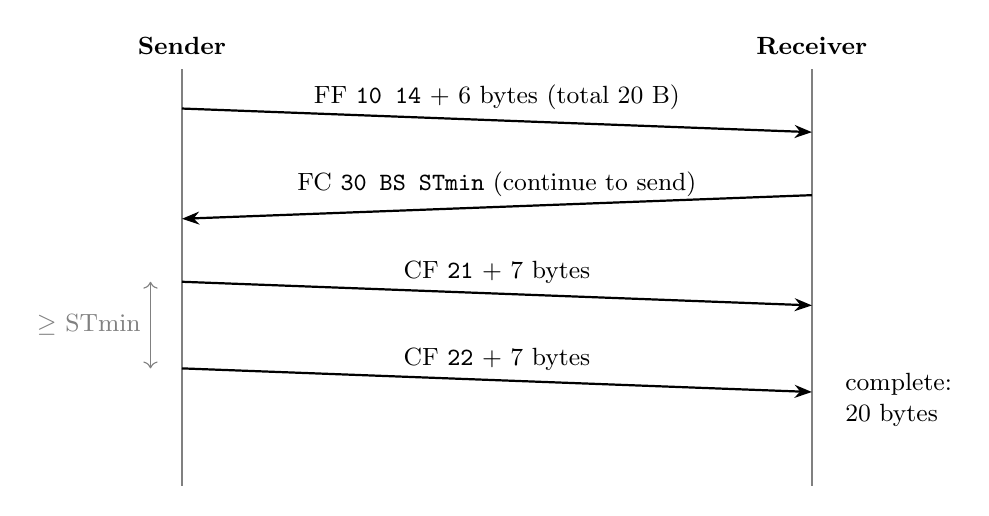
\begin{tikzpicture}[font=\small]
  \node (s) at (0,0) {\textbf{Sender}};
  \node (r) at (8,0) {\textbf{Receiver}};
  \draw[thick,gray] (0,-0.3) -- (0,-5.6);
  \draw[thick,gray] (8,-0.3) -- (8,-5.6);
  \draw[arr] (0,-0.8) -- node[above]{FF \texttt{10 14} + 6 bytes (total 20 B)} (8,-1.1);
  \draw[arr] (8,-1.9) -- node[above]{FC \texttt{30 BS STmin} (continue to send)} (0,-2.2);
  \draw[arr] (0,-3.0) -- node[above]{CF \texttt{21} + 7 bytes} (8,-3.3);
  \draw[arr] (0,-4.1) -- node[above]{CF \texttt{22} + 7 bytes} (8,-4.4);
  \node[align=left,anchor=west] at (8.3,-4.5) {complete:\\20 bytes};
  \draw[<->,gray] (-0.4,-3.0) -- node[left]{$\ge$ STmin} (-0.4,-4.1);
\end{tikzpicture}
\caption{Segmented ISO-TP transfer of a 20-byte message}
\label{fig:isotp_seq}
\end{figure}

\section{Unified Diagnostic Services (ISO 14229)}

UDS defines a request/response protocol between a tester and an ECU~\cite{ISO14229-1}. A request starts with a service identifier (SID); a positive response echoes SID\,+\,0x40, and a negative response is \texttt{7F SID NRC} with a negative response code such as 0x11 (service not supported) or 0x31 (request out of range). The services targeted by this project are Diagnostic Session Control (0x10), ECU Reset (0x11), Clear Diagnostic Information (0x14), Read DTC Information (0x19), Read Data By Identifier (0x22) and Tester Present (0x3E). On vehicles the physical request and response identifiers of the engine ECU are commonly 0x7E0 and 0x7E8; the project reuses this pair.

\section{End-to-End Protection}

Bus-level CAN checks detect transmission errors on the wire but not faults inside an ECU, such as a stuck task that keeps resending an old buffer or corrupted RAM. AUTOSAR E2E profiles therefore add, inside the payload, an alive (sequence) counter and a CRC computed by the sender and verified by the receiver~\cite{AUTOSAR_E2E}. Profile~1 uses a 4-bit counter and CRC-8 SAE-J1850 (polynomial 0x1D)~\cite{SAEJ1850}. The receiver classifies each frame as correct, repeated, with some frames lost, or with a wrong sequence, and discards data that fails the check.

\section{Layered ECU Software}

The AUTOSAR classic platform separates application software from basic software, and at the bottom of the basic software the microcontroller abstraction layer (MCAL) encapsulates all register access~\cite{AUTOSAR_LayeredArch}. This project applies the same idea at a small scale: only MCAL drivers call the STM32 HAL; communication and service modules are portable C.

\section{STM32MP157 Heterogeneous Architecture}

The STM32MP157 combines two Cortex-A7 cores running Linux with a Cortex-M4 microcontroller core~\cite{RM0436}. In the \textit{production} boot mode used here, Linux starts first, owns the clock tree and loads the M4 firmware from the file system through the \texttt{remoteproc} framework. The M4 has no flash of its own; its code runs from internal SRAM and must be reloaded after each power cycle. Peripherals are assigned to one of the cores; a peripheral assigned to the M4 is disabled in the Linux device tree, but its kernel clock is still generated by the reset and clock controller (RCC), whose settings are left by Linux. This division of responsibilities is central to the bring-up issues analysed in Section~\ref{sec:bringup}.

\chapter{SYSTEM DESIGN}
\label{ch:design}

\section{Requirements}

Table~\ref{tab:requirements} lists the requirements derived from the objectives in Chapter~\ref{ch:intro}. They are referenced in the evaluation in Chapter~\ref{ch:discussion}.

\begin{table}[H]
\centering
\small
\caption{System requirements}
\label{tab:requirements}
\begin{tabularx}{\textwidth}{@{}lX@{}}
\toprule
\textbf{ID} & \textbf{Requirement} \\
\midrule
R1 & Classic CAN 2.0A, 11-bit identifiers, 500\,kbit/s, sample point close to 87.5\,\% on every node. \\
R2 & The Sensor ECU publishes the speed signal every 10\,ms and a node heartbeat every 100\,ms. \\
R3 & Cyclic frames carry an alive counter and a CRC; the receiver rejects corrupted, repeated and out-of-sequence data. \\
R4 & The Control ECU detects a missing speed signal within 100\,ms, an out-of-range speed and an E2E error, and then drives its output to a safe state (0\,\%). \\
R5 & Fault injection on both ECUs by push button, without changing wiring. \\
R6 & Diagnostic access through UDS over ISO-TP on 0x7E0/0x7E8, with negative responses. \\
R7 & Only the MCAL layer accesses the HAL; protocol modules are hardware independent and unit tested on a PC. \\
R8 & Bus-off is recovered automatically after a delay, without resetting the ECU. \\
\bottomrule
\end{tabularx}
\end{table}

\section{System Architecture and Hardware}

Figure~\ref{fig:system} shows the target network. Table~\ref{tab:hardware} lists the hardware.

\begin{figure}[H]
\centering
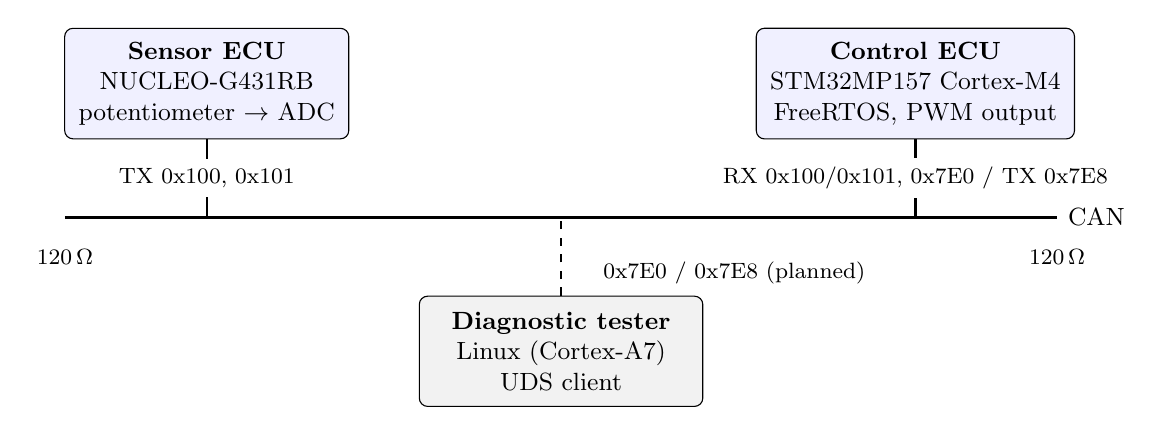
\begin{tikzpicture}[font=\small]
  \node[node] (sen) at (0,0) {\textbf{Sensor ECU}\\NUCLEO-G431RB\\potentiometer $\rightarrow$ ADC};
  \node[node] (ctl) at (9,0) {\textbf{Control ECU}\\STM32MP157 Cortex-M4\\FreeRTOS, PWM output};
  \node[node, fill=gray!10] (tst) at (4.5,-3.4) {\textbf{Diagnostic tester}\\Linux (Cortex-A7)\\UDS client};
  \draw[very thick] (-1.8,-1.7) -- (10.8,-1.7) node[right]{CAN};
  \draw[thick] (sen.south) -- (0,-1.7);
  \draw[thick] (ctl.south) -- (9,-1.7);
  \draw[thick,dashed] (tst.north) -- (4.5,-1.7);
  \node[font=\footnotesize, fill=white] at (0,-1.2) {TX 0x100, 0x101};
  \node[font=\footnotesize, fill=white] at (9,-1.2) {RX 0x100/0x101, 0x7E0 / TX 0x7E8};
  \node[font=\footnotesize] at (6.7,-2.4) {0x7E0 / 0x7E8 (planned)};
  \node[font=\footnotesize,align=center] at (-1.8,-2.2) {120\,$\Omega$};
  \node[font=\footnotesize,align=center] at (10.8,-2.2) {120\,$\Omega$};
\end{tikzpicture}
\caption{Target network architecture. The dashed tester link is future work.}
\label{fig:system}
\end{figure}

\begin{table}[H]
\centering
\small
\caption{Hardware}
\label{tab:hardware}
\begin{tabularx}{\textwidth}{@{}Xp{6.4cm}@{}}
\toprule
\textbf{Item} & \textbf{Use} \\
\midrule
NUCLEO-G431RB (STM32G431RB, Cortex-M4F, 170\,MHz)~\cite{UM2505,RM0440} & Sensor ECU; on-board ST-LINK for flashing and a virtual COM port for logs \\
STM32MP157D-DK1 (2$\times$Cortex-A7 + Cortex-M4)~\cite{UM2637,RM0436} & Control ECU on the M4, Linux (OpenSTLinux, kernel 6.6) on the A7 cores \\
SN65HVD230 3.3\,V CAN transceiver (2$\times$)~\cite{SN65HVD230} & Physical layer; 3.3\,V parts avoid level shifting on 3.3\,V MCU pins \\
10\,k$\Omega$ potentiometer, push buttons, LED + 220\,$\Omega$ & Speed input, fault injection, PWM output \\
USB-to-UART adapter & Log of the M4 firmware (UART7) \\
\bottomrule
\end{tabularx}
\end{table}

\section{CAN Configuration}

\subsection{Bit timing}

The two controllers run from different kernel clocks, so each node has its own timing. Both are derived from a crystal (HSE) because the tolerance bound of Equation~\ref{eq:tolerance} is below 0.5\,\% for both configurations. Table~\ref{tab:bittiming} gives the values.

\begin{table}[H]
\centering
\small
\caption{Bit-timing configuration (500\,kbit/s)}
\label{tab:bittiming}
\begin{tabular}{@{}lcc@{}}
\toprule
 & \textbf{Sensor ECU (STM32G431)} & \textbf{Control ECU (STM32MP157)} \\
\midrule
Kernel clock & 170\,MHz (PCLK1, from 24\,MHz HSE) & 24\,MHz (HSE) \\
Prescaler & 10 & 3 \\
$t_q$ & 58.8\,ns & 125\,ns \\
Seg1 / Seg2 / SJW & 29 / 4 / 4 & 13 / 2 / 2 \\
NBT & 34\,tq & 16\,tq \\
Bit rate & 500\,000\,bit/s & 500\,000\,bit/s \\
Sample point & 88.2\,\% & 87.5\,\% \\
Tolerance bound (Eq.~\ref{eq:tolerance}) & 0.46\,\% & 0.49\,\% \\
\bottomrule
\end{tabular}
\end{table}

On the STM32G431, 170\,MHz cannot be divided into a 16-quantum bit at 500\,kbit/s, so 34\,tq were used; the resulting 88.2\,\% sample point is within a fraction of a quantum of 87.5\,\%. On the STM32MP157 the 24\,MHz HSE gives exactly 16\,tq and 87.5\,\%. The kernel clock that Linux selects by default (PLL4\_R, 74.25\,MHz) cannot produce 500\,kbit/s exactly ($74.25\,\text{MHz}/500\,\text{kHz} = 148.5$); the Control ECU therefore switches the FDCAN kernel clock to HSE at start-up (Section~\ref{sec:bringup}) and keeps a fallback timing for 74.25\,MHz with a 0.34\,\% error.

\subsection{CAN matrix}

Table~\ref{tab:canmatrix} lists the identifiers. The byte layout is defined once in \texttt{common/can/can\_matrix.h}, which both firmware projects compile, so the layouts cannot drift apart. The detailed layout is in Appendix~\ref{app:frames}.

\begin{table}[H]
\centering
\small
\caption{CAN matrix}
\label{tab:canmatrix}
\begin{tabularx}{\textwidth}{@{}llccX@{}}
\toprule
\textbf{ID} & \textbf{Name} & \textbf{Sender} & \textbf{Cycle} & \textbf{Content} \\
\midrule
0x100 & SENSOR\_SPEED & Sensor ECU & 10\,ms & speed (0.1\,km/h), raw ADC, status, alive counter, CRC-8 \\
0x101 & SENSOR\_ALIVE & Sensor ECU & 100\,ms & node state, uptime, bus-off count, alive counter, CRC-8 \\
0x7E0 & UDS request & tester & event & ISO-TP, physical addressing to the Control ECU \\
0x7E8 & UDS response & Control ECU & event & ISO-TP response \\
\bottomrule
\end{tabularx}
\end{table}

Multi-byte signals are big-endian (Motorola byte order), as is usual in automotive signal databases, and the speed is an unsigned integer in 0.1\,km/h so that no floating-point value travels on the bus.

\section{Software Architecture}

Figure~\ref{fig:layers} shows the layering. MCAL drivers wrap the STM32 HAL; everything above them is portable C. The shared modules in \texttt{common/} are linked into both STM32CubeIDE projects as a linked folder, so the firmware and the PC unit tests compile the very same source files.

\begin{figure}[H]
\centering
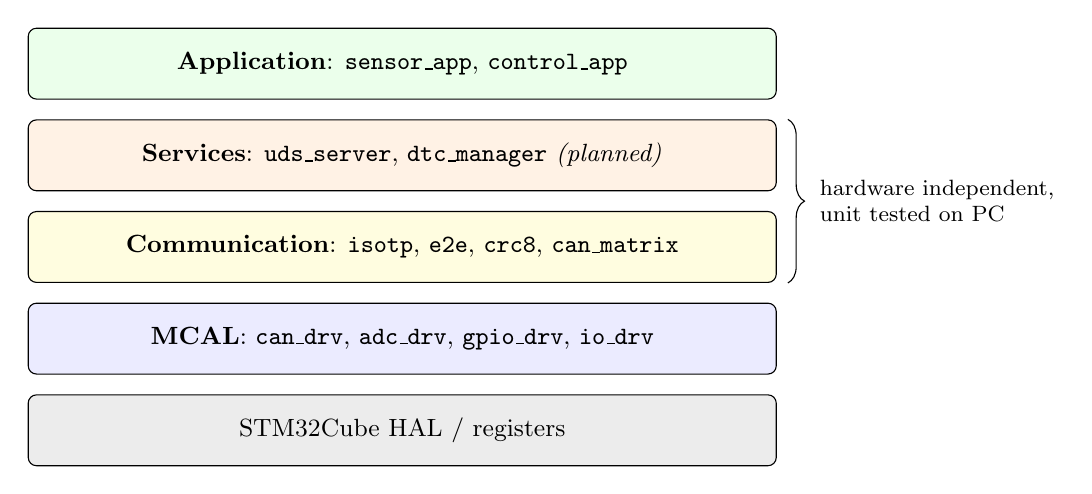
\begin{tikzpicture}[font=\small, node distance=0.25cm]
  \node[layer, fill=green!8] (app) {\textbf{Application}: \texttt{sensor\_app}, \texttt{control\_app}};
  \node[layer, fill=orange!10, below=of app] (svc) {\textbf{Services}: \texttt{uds\_server}, \texttt{dtc\_manager} \textit{(planned)}};
  \node[layer, fill=yellow!12, below=of svc] (com) {\textbf{Communication}: \texttt{isotp}, \texttt{e2e}, \texttt{crc8}, \texttt{can\_matrix}};
  \node[layer, fill=blue!8, below=of com] (mcal) {\textbf{MCAL}: \texttt{can\_drv}, \texttt{adc\_drv}, \texttt{gpio\_drv}, \texttt{io\_drv}};
  \node[layer, fill=gray!15, below=of mcal] (hal) {STM32Cube HAL / registers};
  \draw[decorate,decoration={brace,amplitude=6pt}] ([xshift=4pt]svc.north east) -- ([xshift=4pt]com.south east)
    node[midway,right=8pt,align=left,font=\footnotesize]{hardware independent,\\unit tested on PC};
\end{tikzpicture}
\caption{AUTOSAR-inspired software layers}
\label{fig:layers}
\end{figure}

\section{Sensor ECU Design}

The Sensor ECU runs bare-metal. TIM6 raises a flag every 10\,ms; the main loop consumes it and runs one task cycle. The interrupt routine only sets the flag, so ADC conversions, CAN writes and logging never execute in interrupt context, and a missed deadline is counted as an overrun. Each cycle:
\begin{enumerate}[nosep]
  \item debounces push button B1 (30\,ms) and advances the fault-injection mode on each press;
  \item samples the potentiometer (12-bit ADC, 92.5-cycle sampling time) and filters it with an 8-sample moving average;
  \item scales the value to 0--250.0\,km/h and sends frame 0x100 protected by the E2E module;
  \item every tenth cycle sends frame 0x101;
  \item runs the bus-off recovery state machine and the status LED.
\end{enumerate}

\paragraph{Sampling time.} The potentiometer wiper has a source impedance of up to 2.5\,k$\Omega$ (two 5\,k$\Omega$ halves in parallel). With a sample capacitor of about 5\,pF, reaching 12-bit accuracy needs roughly ten time constants, about 120\,ns, which the default 2.5-cycle sampling time at 42.5\,MHz (59\,ns) does not provide. 92.5 cycles (2.2\,\textmu s) gives a large margin at negligible cost, since only one sample is taken every 10\,ms.

\paragraph{Fault injection.} Button B1 cycles through three modes: \texttt{NONE}; \texttt{SILENT}, which stops frame 0x100 so that the receiver's timeout detection is exercised; and \texttt{OUT\_OF\_RANGE}, which sends 300.0\,km/h. The status byte of 0x100 flags active fault injection so that injected faults can be told apart from real ones in a bus trace.

\paragraph{Bus-off recovery.} On bus-off the FDCAN hardware sets \texttt{CCCR.INIT}. The driver waits 100\,ms and then clears \texttt{INIT}, which starts the standard recovery sequence of 128$\times$11 recessive bits. The delay prevents a faulty node from flooding the bus with error frames.

\section{Control ECU Design}

The Control ECU runs FreeRTOS~\cite{FreeRTOS} on the Cortex-M4. Figure~\ref{fig:ctrl_flow} shows the data flow.

\begin{figure}[H]
\centering
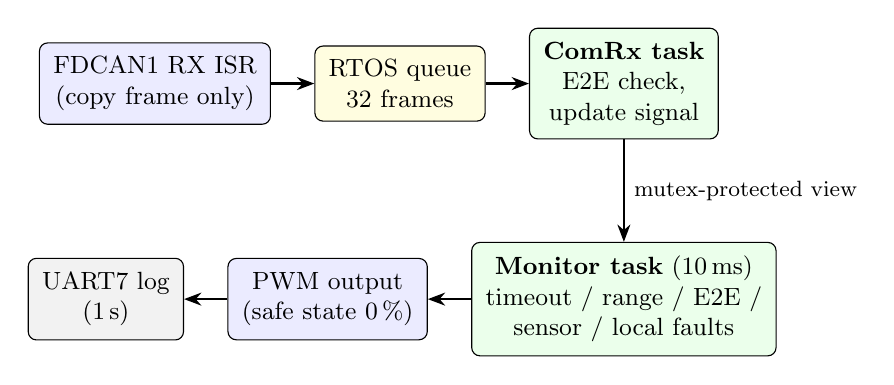
\begin{tikzpicture}[font=\small, node distance=0.55cm]
  \node[box, fill=blue!8] (isr) {FDCAN1 RX ISR\\(copy frame only)};
  \node[box, fill=yellow!12, right=of isr] (q) {RTOS queue\\32 frames};
  \node[box, fill=green!8, right=of q] (com) {\textbf{ComRx task}\\E2E check,\\update signal};
  \node[box, fill=green!8, below=1.3cm of com] (mon) {\textbf{Monitor task} (10\,ms)\\timeout / range / E2E /\\sensor / local faults};
  \node[box, fill=blue!8, left=of mon] (pwm) {PWM output\\(safe state 0\,\%)};
  \node[box, fill=gray!10, left=of pwm] (log) {UART7 log\\(1\,s)};
  \draw[arr] (isr) -- (q);
  \draw[arr] (q) -- (com);
  \draw[arr] (com) -- node[right,font=\footnotesize]{mutex-protected view} (mon);
  \draw[arr] (mon) -- (pwm);
  \draw[arr] (pwm) -- (log);
\end{tikzpicture}
\caption{Control ECU data flow}
\label{fig:ctrl_flow}
\end{figure}

\begin{itemize}
  \item \textbf{Interrupt level.} The FDCAN receive callback copies each frame into an RTOS queue and returns; a full queue is counted rather than blocking.
  \item \textbf{ComRx task} (above-normal priority) runs the E2E check on 0x100, updates a shared view of the sensor signal under a mutex and counts E2E outcomes. Frames 0x7E0/0x7DF are routed to the future UDS server.
  \item \textbf{Monitor task} (normal priority, 10\,ms period with \texttt{osDelayUntil}) evaluates five faults, applies the safe state, runs bus-off recovery and prints a status line every second.
\end{itemize}

Table~\ref{tab:faults} lists the monitored faults. When a fault that invalidates the speed signal is active, the output is forced to 0\,\% instead of using stale or implausible data. The E2E fault heals only after ten consecutive valid frames to avoid chattering.

\begin{table}[H]
\centering
\small
\caption{Faults monitored by the Control ECU}
\label{tab:faults}
\begin{tabularx}{\textwidth}{@{}lXc@{}}
\toprule
\textbf{Fault} & \textbf{Condition} & \textbf{Safe state} \\
\midrule
SPEED\_TIMEOUT & no valid 0x100 for more than 100\,ms (500\,ms grace after start) & yes \\
SPEED\_RANGE & received speed above 250.0\,km/h & yes \\
SPEED\_E2E & CRC or sequence error; healed after 10 valid frames & yes \\
SENSOR\_ADC & Sensor ECU reports an ADC read error in its status byte & no \\
OUTPUT\_LOCAL & toggled by button USER1 (simulated actuator fault) & yes \\
\bottomrule
\end{tabularx}
\end{table}

In a later milestone each fault becomes a DTC with an ISO~14229 status byte in the DTC manager, readable and clearable over UDS.

\section{Communication Modules}

\subsection{E2E protection}

\texttt{E2e\_Protect()} writes the 4-bit alive counter to byte~6 and the CRC-8 SAE-J1850 of bytes 0--6 to byte~7. \texttt{E2e\_Check()} verifies the CRC first, so a corrupted frame never modifies the receiver state, and then classifies the counter difference modulo 16: 0 is \textit{repeated}, 1 is \textit{OK}, 2--3 is \textit{OK with some frames lost}, and larger jumps are rejected as \textit{wrong sequence} with resynchronisation on the next frame.

\subsection{ISO-TP}

The ISO-TP module keeps independent sender and receiver state machines per link. It is hardware independent: the CAN send function and a millisecond clock are injected through a configuration structure, which makes the timing behaviour fully controllable in unit tests. Notable design points:
\begin{itemize}[nosep]
  \item all frames are padded to 8 bytes with 0xCC;
  \item STmin is enforced with one extra tick of margin, because with a 1\,ms clock a frame sent at $x.99$\,ms and the next at $(x+1).00$\,ms would be only 0.01\,ms apart;
  \item STmin values in the 100--900\,\textmu s range are rounded up to 1\,ms, and reserved values are treated as the 127\,ms maximum, as required by the standard;
  \item if the CAN driver is busy (three TX FIFO slots on the STM32), a frame is retried on the next cycle instead of being dropped;
  \item N\_Bs and N\_Cr timeouts, a limit on consecutive FC.WAIT frames and FC.OVFLW handling abort a transfer with an explicit result code.
\end{itemize}

\section{Verification Strategy}

Verification proceeds bottom-up:
\begin{enumerate}[nosep]
  \item \textbf{Unit tests on a PC} for all hardware-independent modules, using a fake CAN driver and a fake clock. Compiled with \texttt{-Wall -Wextra -Wpedantic -Wshadow -Wconversion}.
  \item \textbf{FDCAN internal loopback} on each ECU, which exercises bit-timing configuration, filters, interrupts and the full software path without a transceiver.
  \item \textbf{Two-node bus} with transceivers, checked with a logic analyser (next milestone).
  \item \textbf{System test} with the UDS tester (final milestone).
\end{enumerate}
Each hardware test records the UART log as evidence, together with a pass criterion defined before the run.

\chapter{IMPLEMENTATION AND RESULTS}
\label{ch:results}

\section{Development Environment}

\begin{table}[H]
\centering
\small
\caption{Tools}
\label{tab:tools}
\begin{tabularx}{\textwidth}{@{}lX@{}}
\toprule
\textbf{Tool} & \textbf{Use} \\
\midrule
STM32CubeMX 6.18 & peripheral, clock and middleware configuration of both projects \\
STM32CubeIDE 2.2 / GNU Arm toolchain 14.3 & firmware build \\
STM32CubeProgrammer CLI & flashing the NUCLEO-G431RB over SWD \\
OpenSTLinux (kernel 6.6), \texttt{remoteproc}, SSH over USB & loading and starting the M4 firmware on the DK1 \\
MSYS2 GCC and GNU Make & host unit tests \\
Git / GitHub & version control; each verified milestone is tagged \\
\bottomrule
\end{tabularx}
\end{table}

The M4 firmware is deployed by copying the ELF file to \texttt{/lib/firmware} and writing to the \texttt{remoteproc} sysfs interface (Appendix~\ref{app:procedures}).

\section{Unit Tests}

The hardware-independent modules are tested on a PC with a minimal self-written test harness (no external framework), a fake CAN driver that records every transmitted frame and can simulate a busy driver, and a fake millisecond clock that only advances when a test says so. Table~\ref{tab:unittests} summarises the suites.

\begin{table}[H]
\centering
\small
\caption{Unit test results}
\label{tab:unittests}
\begin{tabularx}{\textwidth}{@{}lccX@{}}
\toprule
\textbf{Suite} & \textbf{Tests} & \textbf{Checks} & \textbf{Scope} \\
\midrule
ISO-TP & 26 & 115 & SF/FF/CF/FC in both directions, padding, block size, STmin in ms and \textmu s encoding, N\_Bs and N\_Cr timeouts, FC.WAIT limit, FC.OVFLW, receive buffer overflow, wrong sequence number, SF interrupting a segmented reception, sequence number wrap-around (200 bytes), driver-busy retry, and a 4095-byte end-to-end transfer between two links on a simulated bus \\
E2E & 8 & 58 & CRC-8 catalogue value (\texttt{"123456789"} $\rightarrow$ 0x4B), counter wrap 15$\rightarrow$0, single-bit corruption, repeated frame, lost frames and resynchronisation, short frame \\
DTC manager & 11 & 35 & status bits after pass/fail, confirmation after consecutive failures with debounce reset, healing keeps history bits, operation-cycle rules for \textit{pendingDTC}, clear, read by status mask, balanced lock callbacks \\
UDS server & 11 & 69 & every service with positive and negative responses, suppress-positive-response bit, S3 session timeout, multi-DID read, response-too-long, reset only in the extended session and only after the response, functional-addressing NRC suppression \\
\midrule
\textbf{Total} & \textbf{56} & \textbf{277} & all pass, 0 failures \\
\bottomrule
\end{tabularx}
\end{table}

The 4095-byte end-to-end test also checks the exact frame count: one first frame, 585 consecutive frames and 74 flow-control frames for a block size of 8. An error in the expected count found while writing this test (584 instead of 585 consecutive frames, because $4089 = 584 \times 7 + 1$) illustrates why such arithmetic belongs in automated tests rather than in comments. Similarly, one DTC test initially expected a DTC with status 0x00 to be reported for the mask 0xFF; ISO~14229 reports a DTC only if \texttt{(status \& mask) != 0}, so the implementation was right and the expectation was corrected.

\section{Milestone M1: Sensor ECU in Loopback}

The Sensor ECU firmware was flashed with the STM32CubeProgrammer CLI and run in FDCAN internal loopback, where the controller receives its own frames. The pass criterion was: transmit rate as designed, every 0x100 frame received back, no dropped frame, no bus-off, and a stable ADC reading that follows the potentiometer. Figure~\ref{fig:m1} shows the log and Table~\ref{tab:m1} the results.

\reportimage{m1_sensor_loopback_uart.png}{0.95}{Sensor ECU log in FDCAN internal loopback (one line per second)}{fig:m1}

\begin{table}[H]
\centering
\small
\caption{Milestone M1 results}
\label{tab:m1}
\begin{tabularx}{\textwidth}{@{}lXc@{}}
\toprule
\textbf{Check} & \textbf{Observation} & \textbf{Result} \\
\midrule
Transmit rate & +110 frames per second (100$\times$0x100 + 10$\times$0x101) & \cmark \\
Loopback reception & \texttt{rx100} +100 per second; \texttt{rx = tx - 2} constant (two frames in flight when the log is printed) & \cmark \\
Endurance & more than 59\,000 frames, \texttt{drop=0}, \texttt{busoff=0} & \cmark \\
ADC & follows the potentiometer (0 to 104.8\,km/h observed during the sweep); $\pm$1--2\,LSB at rest & \cmark \\
Scaling & e.g. ADC 865 $\rightarrow$ $865 \times 2500/4095 = 528$ $\rightarrow$ 52.8\,km/h & \cmark \\
Fault injection (B1) & not yet exercised on hardware & open \\
\bottomrule
\end{tabularx}
\end{table}

\section{Milestone M2: Control ECU in Loopback}

In loopback the Control ECU also plays the Sensor ECU: its monitor task sends an E2E-protected 0x100 frame every 10\,ms with a speed ramp from 0 to 250\,km/h, so the whole chain from the FDCAN interrupt to the PWM output is exercised on the DK1 alone. Figure~\ref{fig:m2} shows the log and Table~\ref{tab:m2} the results.

\reportimage{m2_control_loopback_uart.png}{0.95}{Control ECU log on the STM32MP157 Cortex-M4 in FDCAN internal loopback}{fig:m2}

\begin{table}[H]
\centering
\small
\caption{Milestone M2 results}
\label{tab:m2}
\begin{tabularx}{\textwidth}{@{}lXc@{}}
\toprule
\textbf{Check} & \textbf{Observation} & \textbf{Result} \\
\midrule
Reception & \texttt{e2e ok} +100 per second, \texttt{rx = tx - 1} & \cmark \\
E2E & 30\,900 frames: 0 CRC, 0 lost, 0 repeated, 0 sequence errors & \cmark \\
Signal freshness & \texttt{age = 10\,ms} (timeout threshold 100\,ms) & \cmark \\
Output & PWM tracks speed, e.g. 193.4\,km/h $\rightarrow$ 77.3\,\% & \cmark \\
Faults & timeout active at start-up, cleared automatically once data arrives; no active fault afterwards & \cmark \\
RTOS & 0 queue overflows; 11\,032 bytes of the 16\,KB heap free & \cmark \\
\bottomrule
\end{tabularx}
\end{table}

\section{Milestone M3: UDS and DTC Management on the Control ECU}

The UDS server, the DTC manager and an ISO-TP link were integrated into the Control ECU, and the on-target self-test described in Section~\ref{sec:diag_design} was run in FDCAN internal loopback. Listing~\ref{lst:m3} shows the log; the complete log is stored in the repository (\texttt{docs/logs/m3\_uds\_selftest.log}). All 14 steps passed on the first hardware run.

\begin{lstlisting}[language={},numbers=none,caption={On-target UDS self-test on the Cortex-M4 (UART7 log, abridged)},label={lst:m3}]
[TEST]  1/14 TesterPresent                    PASS
[TEST]  2/14 ReadDID F195 (ECU sends FF+CF)   PASS
[TEST]  3/14 ReadDID x4 (ECU receives FF+CF)  PASS
[TEST]  4/14 Unknown service -> NRC 11        PASS
[TEST]  5/14 Unknown DID -> NRC 31            PASS
[TEST]  6/14 Reset in default -> NRC 7E       PASS
[TEST]  7/14 Session extended                 PASS
[TEST]  8/14 Confirmed DTCs = 0               PASS
[CTRL] fault OUTPUT_LOCAL  SET
[TEST]  9/14 Confirmed DTCs = 1               PASS
[TEST] 10/14 DTC list B1A00-11 0x2F           PASS
[CTRL] fault OUTPUT_LOCAL  cleared
[TEST] 11/14 Clear all DTCs                   PASS
[TEST] 12/14 Confirmed DTCs = 0 again         PASS
[CTRL] soft reset: new operation cycle
[TEST] 13/14 Soft reset                       PASS
[TEST] 14/14 Session default                  PASS
[TEST] UDS self-test finished: 14/14 passed
[CTRL] speed=249.5 km/h age=10ms pwm=99.8% | e2e ok=499 lost=0 crc=0 rep=0
       seq=0 | faults=0x00 dtc=0 | rx=537 tx=538 busoff=0 qovf=0 uds=38 heap=9744
\end{lstlisting}

\begin{table}[H]
\centering
\small
\caption{Milestone M3 results}
\label{tab:m3}
\begin{tabularx}{\textwidth}{@{}lXc@{}}
\toprule
\textbf{Check} & \textbf{Observation} & \textbf{Result} \\
\midrule
Segmented transfers & 13-byte response from the ECU and 9-byte request to the ECU, both with FF/CF and flow control & \cmark \\
Negative responses & NRC 0x11 (unknown service), 0x31 (unknown DID), 0x7E (reset in default session) & \cmark \\
Fault to DTC & local fault injected $\rightarrow$ DTC B1A00-11 confirmed with status 0x2F (TF, TFTOC, PDTC, CDTC, TFSLC) & \cmark \\
Clear & 0x14 FFFFFF $\rightarrow$ no confirmed DTC & \cmark \\
Sessions and soft reset & extended session with P2/P2*, soft reset starts a new operation cycle & \cmark \\
No side effects & 38 diagnostic frames exchanged while sensor data kept flowing: 0 E2E errors, 0 queue overflows; 9.7\,KB heap free & \cmark \\
Hard reset (0x11 01) & cannot be exercised by a tester running on the same core & open \\
\bottomrule
\end{tabularx}
\end{table}

\section{Milestone M4: Two-Node Bus with Fault Injection}

\subsection{Wiring}

Table~\ref{tab:wiring} lists the verified connections. Each transceiver module carries a 120\,$\Omega$ terminator, so the bus measures about 60\,$\Omega$ between CANH and CANL; both boards share a common ground.

\begin{table}[H]
\centering
\small
\caption{Verified bus wiring}
\label{tab:wiring}
\begin{tabularx}{\textwidth}{@{}lXlX@{}}
\toprule
\textbf{Signal} & \textbf{NUCLEO-G431RB} & \textbf{SN65HVD230} & \textbf{STM32MP157D-DK1} \\
\midrule
FDCAN1\_TX & PA12, CN10 pin 12 & CTX & PA12, CN13 pin 9 (Arduino D14) \\
FDCAN1\_RX & PA11, CN10 pin 14 & CRX & PA11, CN13 pin 10 (Arduino D15) \\
Supply & 3V3 / GND (CN6) & 3V3 / GND & CN16 pin 4 / pin 6 \\
\bottomrule
\end{tabularx}
\end{table}

\subsection{Diagnosing the bus bring-up}

The first power-up on the bus did not work, and the fault was located without an oscilloscope by reading the FDCAN status registers of both nodes (the Nucleo through the ST-LINK in hot-plug mode, the DK1 from Linux). The last error code (LEC) of the protocol status register was the key observable:

\begin{enumerate}[nosep]
  \item The Sensor ECU reported LEC\,=\,3 (\textit{acknowledge error}) with its transmit error counter at 128. A node only reaches the acknowledge slot if it has read back every bit it sent, so the path Nucleo\,$\rightarrow$\,transceiver\,$\rightarrow$\,bus\,$\rightarrow$\,transceiver\,$\rightarrow$\,Nucleo was proven; only an acknowledging receiver was missing.
  \item On the DK1 the receive pin PA11, sampled 50\,000 times per second from Linux, never went low while the Nucleo was retransmitting: no signal reached the DK1.
  \item Swapping the two transceiver modules on the Nucleo reproduced LEC\,=\,3 with the second module as well, so both modules were good and the fault was on the DK1 side. The DK1 wires were moved to the documented header pins (CN13 pins 9 and 10).
  \item A cyclic status frame (0x200) was added to the Control ECU so that it also transmits. The DK1 then reported LEC\,=\,3 too: each node read back its own frames, but neither received the other, which located the fault in the link between the two modules; the CANH/CANL wires had been removed during module testing.
  \item After reconnecting, both nodes reported LEC\,=\,5 (\textit{bit-0 error}) and cycled through bus-off. To separate a polarity error from other causes, the DK1 controller was switched to bus-monitoring (listen-only) mode from Linux: it received the Sensor ECU frames with valid E2E checks, which proved the polarity correct. With stable connections the bus then ran without errors.
\end{enumerate}

During this phase the Sensor ECU went through several hundred bus-off events and recovered from each automatically, which exercises requirement R8 on real hardware.

\subsection{Fault injection test}

Both logs were captured simultaneously for 65\,s while the potentiometer was swept and button B1 of the Sensor ECU was used to inject faults. Table~\ref{tab:m4} summarises the run; the complete logs are in \texttt{docs/logs/}.

\begin{table}[H]
\centering
\small
\caption{Milestone M4: fault injection over the physical bus}
\label{tab:m4}
\begin{tabularx}{\textwidth}{@{}lXX@{}}
\toprule
\textbf{Time} & \textbf{Sensor ECU} & \textbf{Control ECU} \\
\midrule
23--33\,s & potentiometer sweep, 142--233\,km/h & received speed and PWM follow \\
39.7\,s & B1: SILENT, frame 0x100 stopped & 39.8\,s: SPEED\_TIMEOUT set, PWM 0\,\%, DTC U0100-87 confirmed \\
46.7\,s & B1: OUT\_OF\_RANGE, 300.0\,km/h sent & timeout cleared, SPEED\_RANGE set, PWM 0\,\%, DTC P0501-00 confirmed \\
55.6\,s & B1: back to normal & SPEED\_RANGE cleared, PWM 64.5\,\% again; confirmed DTCs retained \\
whole run & 110 frames/s, no frame dropped & 100 frames/s, 0 CRC, lost or repeated errors, 0 bus-off, 0 queue overflows \\
\bottomrule
\end{tabularx}
\end{table}

The timeout was reported one log line (100\,ms resolution) after the Sensor ECU changed mode, consistent with the 100\,ms timeout threshold. The DTC count stayed at three after all faults had healed: confirmed DTCs are kept until a tester clears them, as ISO~14229 requires. One of the three, U0400-81, was stored when the bus first came up: the Sensor ECU flushed three stale frames from its transmit FIFO with old alive counters, and the E2E check correctly classified them as out of sequence.

\section{Bring-up of the Control ECU}
\label{sec:bringup}

The first run of the Control ECU on the DK1 did nothing observable. No debugger connection to the M4 was available in production mode (the A7 owns the M4 reset), and the UART log was not yet readable. The firmware state was therefore inspected from Linux, which can read the M4 SRAM (aliased at 0x3002\,0000) and all peripheral registers through \texttt{/dev/mem}; symbol addresses and structure offsets were taken from the ELF file with \texttt{nm} and \texttt{gdb}. Two independent defects were found.

\subsection{Issue 1: missing SysTick handler}

\textbf{Observation.} \texttt{xSchedulerRunning = 1} and the current task was the idle task, but the FreeRTOS tick count \texttt{xTickCount} stayed at 0 and the HAL tick \texttt{uwTick} was frozen at 19. All application tasks were blocked waiting for a tick that never came.

\textbf{Root cause.} STM32CubeMX generated \texttt{USE\_CUSTOM\_SYSTICK\_HANDLER\_IMPLEMENTATION = 1}, which tells the CMSIS-RTOS2 layer not to define \texttt{SysTick\_Handler} because the interrupt file will. With TIM7 selected as HAL time base, however, the interrupt file contained no such handler. The symbol table showed \texttt{SysTick\_Handler} as a weak alias of \texttt{Default\_Handler}, an endless loop: the first RTOS tick trapped the CPU at the SysTick priority, which also blocked the TIM7 interrupt and froze \texttt{uwTick}.

\textbf{Fix.} The flag is overridden to 0 inside a \texttt{USER CODE} section of \texttt{FreeRTOSConfig.h}, which STM32CubeMX preserves on regeneration, so that \texttt{cmsis\_os2.c} provides the standard handler. After the fix the symbol is a strong definition and the tick advances at 1\,kHz.

\subsection{Issue 2: FDCAN kernel clock stuck in a glitch-free multiplexer}

\textbf{Observation.} After the first fix the tasks ran, but \texttt{CCCR.INIT} remained 1, no frame was transmitted and the HAL state was \texttt{BUSY} with no error code, meaning that \texttt{HAL\_FDCAN\_Start()} had succeeded. Clearing \texttt{INIT} directly from Linux had no effect either, which pointed to a missing protocol clock rather than to the firmware.

\textbf{Investigation.} Register reads after a fresh Linux boot showed the state left by Linux (Table~\ref{tab:clockstate}). The clock calibration unit of FDCAN1 was in bypass (\texttt{CCFG.BCC = 1}) and therefore not involved.

\begin{table}[H]
\centering
\small
\caption{FDCAN clock state left by Linux after boot}
\label{tab:clockstate}
\begin{tabularx}{\textwidth}{@{}llX@{}}
\toprule
\textbf{Register field} & \textbf{Value} & \textbf{Meaning} \\
\midrule
\texttt{RCC\_FDCANCKSELR} & 3 & FDCAN kernel clock taken from PLL4\_R \\
\texttt{RCC\_PLL4CR.DIVREN} & 0 & PLL4\_R output disabled (unused by Linux) \\
\texttt{RCC\_OCENSETR.HSEKERON} & 0 & HSE kernel clock output not enabled \\
\texttt{RCC\_TZCR.TZEN} & 1 & RCC in secure mode; oscillator \textit{disable} register is secure-only \\
\bottomrule
\end{tabularx}
\end{table}

\textbf{Root cause.} STM32 kernel clock multiplexers are glitch-free: a switch completes only while both the current and the new input are running~\cite{RM0436}. The firmware switched the multiplexer from PLL4\_R to HSE while PLL4\_R was disabled, so the switch never completed and the FDCAN core was left without any clock. The hypothesis was confirmed experimentally: enabling PLL4\_R for a few milliseconds from Linux immediately let \texttt{INIT} clear and frames flow; PLL4\_R was then disabled again and FDCAN kept running from HSE.

\textbf{Fix.} \texttt{CanDrv\_PrepareKernelClock()}, called before the HAL initialises FDCAN, sets the HSE kernel clock enable, temporarily enables the output of the currently selected PLL if it is off, switches to HSE, waits 1\,ms, restores the PLL output exactly as Linux left it, and reads back the effective kernel frequency. The fix was verified after a fresh reboot with no manual register access: the firmware alone brought FDCAN up at 24\,MHz.

\subsection{Other observations}

\begin{itemize}
  \item \textbf{FreeRTOS heap.} The default 3\,KB heap was too small for five tasks (three application tasks plus the idle and timer-service tasks) with newlib re-entrancy enabled; it was raised to 16\,KB, of which 11\,KB remain free.
  \item \textbf{DLC encoding.} The STM32MP1 HAL encodes the data length in bits 19:16 of the header word, whereas the STM32G4 HAL uses the plain byte count. A compile-time assertion in each driver guards against silently using the wrong encoding.
  \item \textbf{HAL tick rate.} In production mode the HAL tick driven by TIM7 runs at about 2\,kHz, because the timer clock configured by Linux differs from the value assumed by STM32CubeMX. The application uses the FreeRTOS tick, which is correct; the HAL tick is an open point.
\end{itemize}

\section{Resource Usage}

\begin{table}[H]
\centering
\small
\caption{Memory footprint (Debug builds)}
\label{tab:memory}
\begin{tabular}{@{}lrrl@{}}
\toprule
\textbf{Firmware} & \textbf{Code} & \textbf{RAM (data+bss)} & \textbf{Available} \\
\midrule
Sensor ECU (STM32G431) & 31.6\,KB & 2.5\,KB & 128\,KB flash / 32\,KB RAM \\
Control ECU (M4, \texttt{-O0}, with UDS/DTC) & 76.5\,KB & 24.8\,KB & 128\,KB code SRAM / 128\,KB data SRAM \\
\bottomrule
\end{tabular}
\end{table}

\chapter{DISCUSSION AND EVALUATION}
\label{ch:discussion}

\section{Evaluation against the Requirements}

Table~\ref{tab:reqeval} maps the results of Chapter~\ref{ch:results} to the requirements of Table~\ref{tab:requirements}. A requirement is marked as met only if it was demonstrated on hardware or by an automated test.

\begin{table}[H]
\centering
\small
\caption{Requirement coverage}
\label{tab:reqeval}
\begin{tabularx}{\textwidth}{@{}lXl@{}}
\toprule
\textbf{ID} & \textbf{Evidence} & \textbf{Status} \\
\midrule
R1 & Different kernel clocks and time-quanta counts on the two nodes; error-free exchange at 500\,kbit/s on the physical bus (M4) & met \\
R2 & M1: 100 + 10 frames per second & met \\
R3 & E2E unit tests; M2: 30\,900 frames checked & met \\
R4 & M4: timeout detected within about 100\,ms and out-of-range immediately, output forced to 0\,\%; E2E detection shown with stale frames & met \\
R5 & Sensor ECU button B1 over the bus (M4); Control ECU local fault through the M3 self-test & met \\
R6 & UDS over ISO-TP on 0x7E0/0x7E8 with NRCs: 22 unit tests and 14/14 on-target self-test (loopback); hard reset not yet exercised & met (loopback) \\
R7 & Only MCAL files include the HAL; 34 PC unit tests on the shared modules & met \\
R8 & Hundreds of bus-off events during bus bring-up, each recovered automatically & met \\
\bottomrule
\end{tabularx}
\end{table}

\section{What Loopback Tests Do and Do Not Prove}

Internal loopback validates a large part of the design: the controller configuration, the acceptance filters, the interrupt path, the frame packing, the E2E protection and the application logic. It does not validate the physical layer. In internal loopback the controller acknowledges its own frames, so an error in the transceiver wiring, the termination, or a mismatch in bit timing between the two nodes would stay invisible. The two ECUs deliberately use different kernel clocks and different numbers of time quanta; whether they interoperate is what milestone M4 then showed on the physical bus; a logic-analyser measurement of the bit time and sample point would complete the picture.

\section{Lessons Learned}

\paragraph{Generated code is part of the system under test.} The SysTick defect came from STM32CubeMX output, not from application code. It was only found because the investigation did not stop at ``the tasks do not run'' but checked the symbol table: a weak symbol resolved to \texttt{Default\_Handler} is a concrete, checkable fact. Putting the fix in a user section of the generated file keeps it across regeneration.

\paragraph{On a heterogeneous SoC the M4 inherits the clock tree of Linux.} Code that works on a standalone MCU can fail on the STM32MP1 because peripherals assigned to the M4 still depend on clock settings chosen by Linux. The FDCAN defect was a consequence of a general hardware rule (glitch-free multiplexers need both inputs running) meeting a specific software state (an unused PLL output switched off). The clean long-term solution is to let Linux configure the FDCAN kernel clock through the device tree; the firmware-side switch with read-back is a pragmatic and verified workaround.

\paragraph{Testing the integration, not only the units.} The unit tests showed that the UDS server and the DTC manager behave as specified in isolation. The on-target self-test added what they cannot show: that ISO-TP runs correctly from an RTOS task fed by an interrupt queue, that two tasks can share the CAN transmitter, and that a fault detected by the monitor is visible over UDS with the right status bits. Running the tester on the ECU itself made this possible before a second node exists.

\paragraph{Error counters as a measuring instrument.} Without an oscilloscope, the CAN controller itself was the most informative instrument during the bus bring-up. An acknowledge error proves that a node reads back its own bits, a bit-0 error that the bus does not become dominant, and listen-only mode separates receiving from transmitting. Swapping modules between known-good positions then isolated each segment of the chain in a few minutes.

\paragraph{Debugging without a debugger.} Reading M4 memory and peripheral registers from Linux through \texttt{/dev/mem}, guided by symbol addresses from the ELF file, proved to be an effective technique on this platform, and it also allowed hypotheses to be tested by writing registers (for example enabling PLL4\_R to confirm the multiplexer theory) before changing any firmware.

\paragraph{Evidence before conclusions.} Several intermediate hypotheses during bring-up were wrong: USB cables and adapters were suspected while simply re-seating the connectors resolved the connection problems, the clock calibration unit was suspected but found in bypass, and the role of the HSE kernel-clock gate could not be isolated because its disable register is secure-only. Recording which observations support each conclusion (Section~\ref{sec:bringup}) keeps the report honest about what was actually proven.

\section{Limitations}

\begin{itemize}
  \item The bit timing on the bus has not been measured with a logic analyser; correctness is inferred from error-free operation.
  \item Diagnostics are verified only against a tester on the same core; an external tester on a physical bus is still missing, and the hard reset has not been exercised.
  \item DTCs are kept in RAM only (no non-volatile storage, no aging).
  \item The HAL tick of the M4 runs at about twice the intended rate in production mode.
  \item The FDCAN clock is reconfigured by the M4 rather than by the Linux device tree.
  \item MISRA compliance is checked with the rule subset that cppcheck can decide; there is no certified checker and no manual review of the undecidable rules. The firmware has not been measured for worst-case execution time or interrupt latency.
\end{itemize}

\chapter{CONCLUSION AND FUTURE WORK}
\label{ch:conclusion}

\section{Conclusion}

This report presented the design of a miniature automotive ECU network and the completion of its first two milestones. A Sensor ECU on an STM32G431 publishes an end-to-end protected speed signal at 500\,kbit/s with the designed timing, and a Control ECU on the Cortex-M4 of an STM32MP157 receives it under FreeRTOS, checks it, supervises it for faults and drives a safe-state output. The protocol layer is portable and backed by 34 passing unit tests, including a full-length ISO-TP transfer. Both ECUs were verified on hardware in internal loopback with zero communication errors over tens of thousands of frames.

The most instructive part of the work was the bring-up of the Control ECU on a heterogeneous SoC, where two defects outside the application code, a missing interrupt handler in generated code and a clock multiplexer blocked by the clock state left by Linux, were located by reading the running firmware's memory and registers from Linux and were fixed in a way that survives code regeneration and a cold boot.

\section{Future Work}

\begin{enumerate}
  \item \textbf{M3 -- physical bus.} Connect both ECUs through SN65HVD230 transceivers with 120\,$\Omega$ termination at both ends, verify the 60\,$\Omega$ bus resistance, and measure bit time and sample point with a logic analyser. Exercise fault injection, timeout and bus-off recovery on the real bus.
  \item \textbf{UDS server.} Implement services 0x10, 0x11, 0x14, 0x19, 0x22 and 0x3E with negative responses and session timing on top of the existing ISO-TP module, with unit tests on the PC.
  \item \textbf{DTC manager.} Store faults as DTCs with ISO~14229 status bits, confirmation and healing counters, readable and clearable over UDS.
  \item \textbf{Tester.} A Python UDS client on Linux using SocketCAN, either through a USB-CAN adapter or the second FDCAN controller of the STM32MP157.
  \item \textbf{Quality.} Static analysis with cppcheck and MISRA rules, a fix for the HAL tick rate, and moving the FDCAN clock configuration into the Linux device tree.
  \item \textbf{Documentation.} A demonstration video of the complete fault-to-DTC-to-tester flow.
\end{enumerate}

\printbibliography[title={REFERENCES}]
\addcontentsline{toc}{chapter}{REFERENCES}
\begin{appendices}
  \chapter{Frame Layouts}
\label{app:frames}

All multi-byte values are big-endian. Bytes 6 and 7 of the cyclic frames are written by \texttt{E2e\_Protect()} and checked by \texttt{E2e\_Check()}.

\begin{table}[H]
\centering
\small
\caption{Frame 0x100 SENSOR\_SPEED (DLC 8, 10\,ms)}
\label{tab:frame100}
\begin{tabularx}{\textwidth}{@{}clX@{}}
\toprule
\textbf{Byte} & \textbf{Signal} & \textbf{Encoding} \\
\midrule
0--1 & VehicleSpeed & unsigned, 0.1\,km/h per bit, valid 0--2500 \\
2--3 & AdcRaw & 12-bit raw ADC value (diagnostic) \\
4 & Status & bit 0: fault injection active; bit 1: ADC read error \\
5 & -- & reserved, 0 \\
6 & AliveCounter & 0--15 in the low nibble, +1 per frame \\
7 & CRC & CRC-8 SAE-J1850 (poly 0x1D, init 0xFF, xor-out 0xFF) over bytes 0--6 \\
\bottomrule
\end{tabularx}
\end{table}

\begin{table}[H]
\centering
\small
\caption{Frame 0x101 SENSOR\_ALIVE (DLC 8, 100\,ms)}
\label{tab:frame101}
\begin{tabularx}{\textwidth}{@{}clX@{}}
\toprule
\textbf{Byte} & \textbf{Signal} & \textbf{Encoding} \\
\midrule
0 & NodeState & 0 = normal, 1 = fault injection \\
1--4 & Uptime & seconds since reset \\
5 & BusOffCount & saturates at 255 \\
6 & AliveCounter & as above \\
7 & CRC & as above \\
\bottomrule
\end{tabularx}
\end{table}

\section*{Example}
A speed of 123.4\,km/h with ADC value 2021, no status flags and alive counter 5 gives the bytes \texttt{04 D2 07 E5 00 00 05 CRC}, where \texttt{0x04D2} = 1234 and \texttt{0x07E5} = 2021.

  \chapter{Build, Deployment and Diagnosis Procedures}
\label{app:procedures}

\section{Host unit tests}

\begin{lstlisting}[language=bash,numbers=none,caption={Running the unit tests}]
cd tests
make            # builds and runs test_isotp and test_e2e
\end{lstlisting}
On Windows the MSYS2 UCRT64 \texttt{gcc} and \texttt{make} must be on the \texttt{PATH}; the makefile detects MinGW and disables the undefined-behaviour sanitiser, which MinGW does not provide.

\section{Sensor ECU}

The project in \texttt{sensor\_ecu/} is built in STM32CubeIDE and flashed through the on-board ST-LINK, for example:
\begin{lstlisting}[language=bash,numbers=none,caption={Flashing the NUCLEO-G431RB}]
STM32_Programmer_CLI -c port=SWD mode=UR -w Debug/sensor_ecu.elf -v -rst
\end{lstlisting}
The log is printed on the ST-LINK virtual COM port at 115200\,baud, 8N1.

\section{Control ECU (Cortex-M4 on the DK1)}

The DK1 boots Linux from the SD card with both BOOT switches ON. Connected to the PC through the USB-C OTG port, it exposes a network interface and is reachable at \texttt{192.168.7.1}.
\begin{lstlisting}[language=bash,numbers=none,caption={Loading and starting the M4 firmware}]
scp control_ecu_CM4.elf root@192.168.7.1:/lib/firmware/control_ecu.elf
ssh root@192.168.7.1
R=/sys/class/remoteproc/remoteproc0
echo control_ecu.elf > $R/firmware
echo start > $R/state          # "stop" to halt the M4
\end{lstlisting}
The M4 log is printed on UART7 (Arduino connector D1 = TX, D0 = RX) at 115200\,baud.

\section{Reading M4 memory and registers from Linux}

The technique used in Section~\ref{sec:bringup}: find the address of a variable in the ELF file, translate the M4 SRAM address (0x1002\,xxxx) to the physical alias seen by the A7 (0x3002\,xxxx) and read it through \texttt{/dev/mem}.
\begin{lstlisting}[language=bash,numbers=none,caption={Locating symbols and structure offsets}]
arm-none-eabi-nm control_ecu_CM4.elf | grep -E " (xTickCount|hfdcan1)$"
arm-none-eabi-gdb -batch -ex "print/x (int)&hfdcan1.State - (int)&hfdcan1" control_ecu_CM4.elf
\end{lstlisting}
\begin{lstlisting}[language=Python,numbers=none,caption={Reading a 32-bit value from M4 SRAM or a peripheral (run on the DK1)}]
import mmap, os, struct
fd  = os.open("/dev/mem", os.O_RDONLY | os.O_SYNC)
ram = mmap.mmap(fd, 0x10000, mmap.MAP_SHARED, mmap.PROT_READ, offset=0x30020000)
can = mmap.mmap(fd, 0x1000,  mmap.MAP_SHARED, mmap.PROT_READ, offset=0x4400E000)
rd  = lambda m, off: struct.unpack("<I", m[off:off + 4])[0]
print("xTickCount =", rd(ram, 0x10025104 - 0x10020000))
print("FDCAN CCCR = 0x%08x" % rd(can, 0x18))
\end{lstlisting}
Peripheral registers of a stopped M4 may be unclocked; reading them then raises a bus error. Oscillator-disable registers of the RCC are secure-only when \texttt{RCC\_TZCR.TZEN = 1} and cannot be written from Linux.

\end{appendices}
\end{document}
